% Midterm Progress Report
% CS 463 - CS Senior Capstone
% Spring 2018
% Authors: Connor Christensen, Lily Shellhammer, William Buffum
\documentclass[draftclsnofoot,onecolumn,letterpaper,10pt,compsoc]{IEEEtran}

% Packaging
\usepackage{geometry}
\usepackage{hyperref}
\usepackage{titling}
\usepackage{color}
\usepackage{listings}
\usepackage{cite}
\usepackage{pdfpages}
\usepackage{pdflscape}
\usepackage{url}
\usepackage{array}
\usepackage{graphicx}
\usepackage{subfig}

\definecolor{lightgray}{rgb}{0.95,0.95,0.95}
\definecolor{darkgray}{rgb}{0.5,0.5,0.5}
\definecolor{softred}{rgb}{0.7,0,0}

\lstdefinelanguage{JavaScript}{
  keywords={typeof, new, true, false, catch, function, return, null, catch, switch, var, if, in, while, do, else, case, break},
  keywordstyle=\color{blue}\bfseries,
  ndkeywords={class, export, boolean, throw, implements, import, this},
  ndkeywordstyle=\color{darkgray}\bfseries,
  identifierstyle=\color{black},
  sensitive=false,
  comment=[l]{//},
  morecomment=[s]{/*}{*/},
  commentstyle=\color{purple}\ttfamily,
  stringstyle=\color{red}\ttfamily,
  morestring=[b]',
  morestring=[b]"
}

\lstset{
   language=JavaScript,
   backgroundcolor=\color{lightgray},
   extendedchars=true,
   basicstyle=\footnotesize\ttfamily,
   showstringspaces=false,
   showspaces=false,
   numbers=left,
   numberstyle=\footnotesize,
   numbersep=9pt,
   tabsize=2,
   breaklines=true,
   showtabs=false,
   captionpos=b
}

\lstdefinelanguage{Stylus}{
  keywords={@media},
  keywordstyle=\color{blue}\bfseries,
  ndkeywords={px},
  ndkeywordstyle=\color{softred}\bfseries,
  identifierstyle=\color{black},
  sensitive=false,
  comment=[l]{//},
  morecomment=[s]{/*}{*/},
  commentstyle=\color{purple}\ttfamily,
  stringstyle=\color{red}\ttfamily,
  morestring=[b]',
  morestring=[b]"
}

\lstset{
   language=Stylus,
   backgroundcolor=\color{lightgray},
   extendedchars=true,
   basicstyle=\footnotesize\ttfamily,
   showstringspaces=false,
   showspaces=false,
   numbers=left,
   numberstyle=\footnotesize,
   numbersep=9pt,
   tabsize=2,
   breaklines=true,
   showtabs=false,
   captionpos=b
}

% Paper type
\geometry{letterpaper, margin=.75in}

% Title page
\title{CS 463 - CS Senior Capstone
	\\Spring 2017
	\\Midterm Progress Report
}

\author{
	Connor I. Christensen \\
	\texttt{chriconn@oregonstate.edu}
	\\
	Lily M. Shellhammer \\
	\texttt{shellhal@oregonstate.edu}
	\\
	William B. Buffum \\
	\texttt{buffumw@oregonstate.edu}
}

\begin{document}
\begin{titlingpage}
    \maketitle
    \begin{abstract}
			Ninkasi Brewing Company is based in Eugene, Oregon, producing and distributing nearly 100,000 barrels of beer each year across the United States and Canada.
			Ninkasi currently tracks brewery data using digital spreadsheets, a laborious, time consuming, and error prone process.
			Quality brewing requires the company to be detail-oriented, organize its data and provide timely actions in the brewing process.
			In order to maintain good quality control in their product and give the company room to scale in its production, our team has been tasked with creating software that will improve the process of entering, storing and accessing data related to the brewing process.
			This document examines work completed on the project to this date.
			At this point in the middle of the winter term, our product has reached an alpha state and has a working interface with no database connections.
			//TODO : ABOUT THIS REPORT
			\\
			\textbf{Keywords:} Brewing, Operations Management, Web App
    \end{abstract}
		\pagebreak
		\tableofcontents
\end{titlingpage}

% briefly recaps the project purposes and goals
% describes where you are currently on the project
% describes what you have left to do
% describes any problems that have impeded your progress, with any solutions you have
% includes particularly interesting pieces of code (if coding is involved)
    % Example set language to javascript
    % \lstset{language=JavaScript}
    % Example include a file with code in it
    % \lstinputlisting{mobile.js}
% includes images of your project -- screen shots, photos, whatever is appropriate
    % Example include an image
    % \centerline{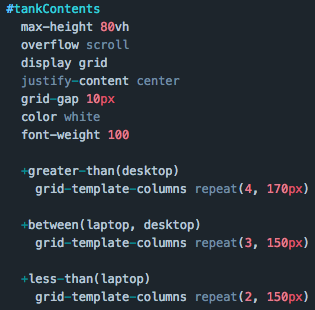
\includegraphics[height=5cm]{screenshots/stylus.png}}

\section{Introduction}
Our team has created a data management web app for Ninkasi Brewing Company.
Ninkasi is a large craft brewery located in Eugene, Oregon that experienced exponential growth in recent years.
The brewing capacity has grown but the data managment technology remains antiquated.
Their outdated data entry system needed to be replaced, and our capstone team worked to create an alternative system.
In the last few weeks, we have finished a beta version of a web app that will serve as an efficient, modern data managment system.
\subsection{Purpose}
The purpose of this document is to outline what we have completed in the first half of our spring term.
We have finished the beta version of product and outline it's progress and challenges in this document.
\subsection{Scope}
This document outlines the role of each member of the team and their progress.
It also discusses future work and interesting code snippets.
\subsection{Overview}
We have reached beta version of our web app and sent a trial version to our client to test out in the brewery.
Our UI and database are nearly complete.
The functionality to check tank statuses, view batch history, enter cellaring data, and view graphs of data over time have all been implemented and have few bugs.
With the exception of a few bugs, we have met our project goals and some of our stretch goals.
\section{Connor Christensen}
\subsection{Current position in the project timeline}

My work has been to build a user interface and assist Lily and Billy with whatever they need to get the project finished.
The user interface is a smaller amount of work for the project, so it was agreed to that I would help out with whatever needed to be done to get the application to a functional level.
The majority of my assistance was going to be towards the work that Lily was doing with Vue.
js, as it is the largest amount of working project.
Over this term I have spent roughly half of my time working on additional requests from the clients and half of the time assisting my teammates with their work.


On April 20th, our group drove down to Ninkasi's headquarters in Eugene and did a final demonstration of the project.
Upon a demo of our project, the client realized that there was some missing functionality that would make their use of the project difficult, as well as some additional utilities that would improve the functionality for the brewers.
The client asked if it would not be too much of a bother to implement them.
It seemed well within our reach, so those tasks were added to our project.


Over the last two weeks, we have been implementing those features as well as bug fixing.
After the demo, our client asked if we could provide them with a functional version of the application for them to test.
I believed that that was possible within the next week.
Unfortunately, it took us a little longer than expected, and the project was released shortly before this midterm progress report.
We have yet to get any feedback from our client or the brewers at Ninkasi, but we look forward to what have to say.



\subsection{What is left to do}

Our team has met all of the minimum requirements for the project as well as several stretch goals outlined in our documentation.
As such, there are no official requirements left for us to fulfill on the development side.
Outlined in our documentation are a few requirements of approval from the brewers on the design and functionality for application, but we will get that from them after they have an opportunity to test our project.


In regard to the course curriculum, the only thing we have left is to make a few revisions to the documentation written over the fall term and submit those changes to both the client and the instructors of the course.
The changes in the documentation are somewhat minor, the biggest diversion being use of different technologies in certain aspects of the site development.



\subsection{Problems encountered and solutions to those problems}

This problem that our team faced This term was dealing with our production database.
Since we had no database for us to tester application locally, we ended up writing junk data into our production database and interfering with each other’s work on a regular basis.
There was some data that persisted from earlier implementations of the database where he did it was not capable of being deleted by anyone other than Billy, so there were a few blocking issues where the database needed to be destroyed and rebuilt before we could properly test.


I found a solution to this issue with configuration of web pack environments.
Web pack has the ability to specify environment variables that are accessible throughout the entire application on compilation.
These environment variables can be a differentiated between the production and development versions of the website.
So, well we were developing the application, we could interact with a local version of the database, specified through the environment variables in the development environment, and when we were ready we could type a single command in the terminal to switch our environments to the production mode.
This gives the flexibility to test the database whenever we wanted without any outside interference.
Each person was capable of is trying and rebuilding the database at any point in time, and the site runs faster without the need to make network requests to a heroku server.


The solution to this problem has an added benefit of not needing a network connection to be able to demo at expo in mid-May.
Both the user interface and the server can be run locally on the computer, without a need for any network requests.


\subsection{Particularly interesting pieces of code}

The most interesting piece of code written or last few weeks has been the user interface surrounding the data entry field on the homepage.
On our trip down to Ninkasi the client asked if it was possible to maintain the labels on the input field even after information had been entered into those fields.
The system in place at the time, was placeholders that defines what information should go and which field.
I was able to find a solution that required a minimal amount of coding and delivered professional looking results on the interface.
Given HTML5’s ability to differentiate between input fields that have user focus and input fields that have been successfully filled in, a minimal amount of CSS is required to be able to make the label dynamically react to the content.

\centerline{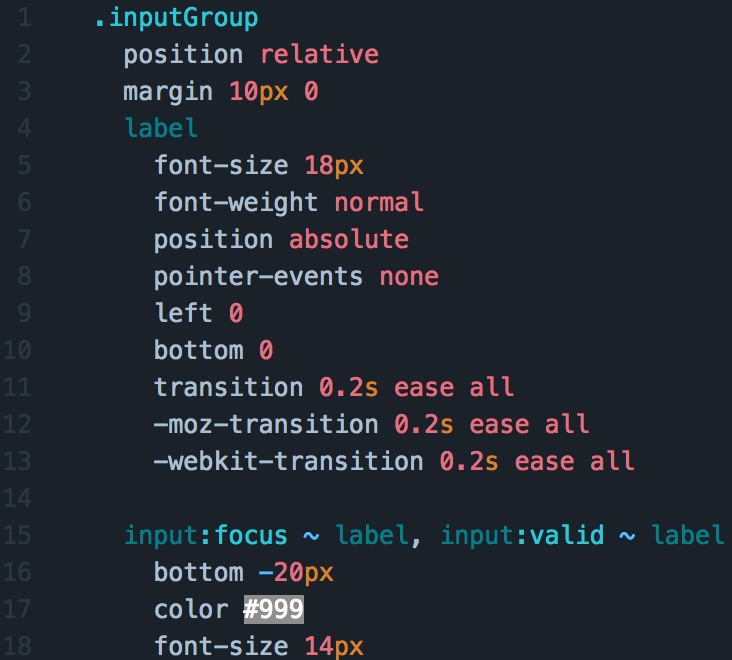
\includegraphics[height=7cm]{screenshots/inputLabel.png}}



\section{Lily Shellhammer}
\subsection{Describe where you are currently on the project}
I have reached beta version for the middle stack.
With the exception of a two bugs, our project is essentially finished.
At the end of last term, we had a few pillars of the site's javascript finished, but we were far from giving our client access to our site.
Since then, I (with some help from my teammates) have finished the following:
\begin{itemize}
\item Submit a new recipe on the admin page
\item Change tanks and actions input to drop down menus
\item Pull most recent data from that tank and auto-populate the form
\item Pull most recent data from tank for tank-info page
\item Edit tank status on the admin page
\item Show given names and airport codes instead of database ids
\item Add new form options to submissions (pressure, bright)
\item Have boxes display actions and colors correctly
\item Create tasks on admin page
\item Take out system of relying on version numbers and compare most recent values
\item Add labels to data entry form boxes
\end{itemize}
The majority of the work this term has been focused on the data entry, tank monitoring, and individual tank view pages.
These are important pages not only because they are the most used, but because they have the most complicated code.
In all of these pages we are pulling the most recent information for a batch given a tank number.
We have to pull the tank information, pull the batch infomration, then find the batch associated with the tank.
Then we pull the batch contents version information, find the batch associated with the tank, and pull the reading with the most recent datestamp.
Then we iterate through the task and actions pages to find if there are any actions needed on specific batches.
\\
Firstly, on the data entry page we utilize this process to pull most recent data so that the brewers don't have to retype measurements that don't often change.
On our tank monitoring page, this process pulls the most recent measurements and actions so that we can display them on small boxes, giving the brewer and overview of measurements and batch statuses.
And finally on our individual tank view page, the most recent readings for every data point are displayed using this process.
\\

\subsection{Describe what you have left to do}
We have two main issues to fix. One is updating the actions of a tank.
We currently can only set the task to a certain action and cannot change that entry.
By adding another action we are able to change the color of the tank as it is associated with a new action, but we cannot edit an old action.
\\
The other issue is submitting a recipe.
We currently submit only a JSON string with the ingredient names specified, not the rates.
This is a difficult fix for me as I don't fully understand how to compound objects or append to them and am struggling the right information online.
\subsection{Describe any problems that have impeded your progress, with any solutions}
Naming was the largest bug creator for me.
There are names in the database that were specifically chosen so as to streamline the whole system's naming, yet conflict with terminology we were originally using.
Because the code has been evolving and changing names with the updating of our database, we often got in trouble where we hadn't updated all the names, yet the old names corresponded to new values so no errors were thrown.
\subsection{Include particularly interesting pieces of code}
One cool feature we implemented is on our data submission page, where we have a drop down menu for the tanks.
When a tank is chosen, we implemented a feature that auto-populates the form with the most recent data taken on those tanks.
This is because there are measurements that don't change much, so we let the brewer use old data and not have to retype everything.
\begin{figure}
  \centering
  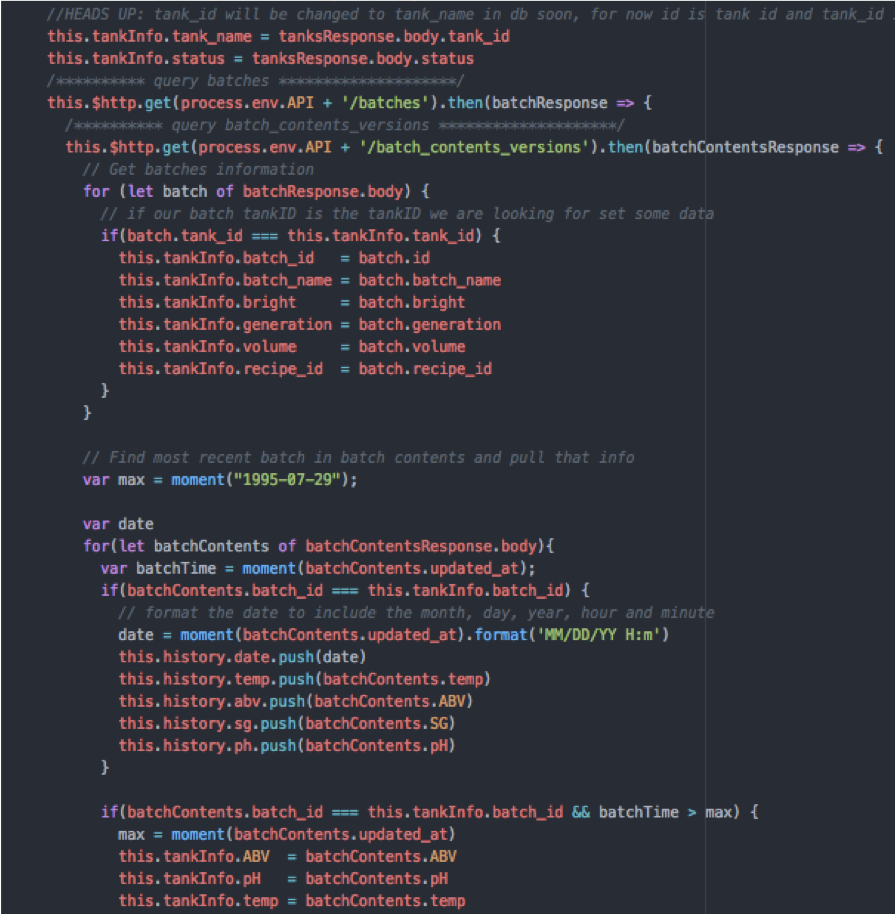
\includegraphics[height=10cm]{screenshots/lily/lilysCode.png}
  \caption{The code used to auto-populate the form with the most recent data}
\end{figure}


\section{William Buffum}
\subsection{Current position in the project timeline}
At the moment, the server is in full beta.
I have the database completed with each necessary table and the REST API to access the database is working.
The server and database are hosted on Heroku so that client side applications can access a stable version.
There are several bugs in the server code and many inefficiencies that will need to be fixed going forward.
I'm pretty happy with the current progress of the server-side code.
As we near the end of the term, Connor, Lily and I are beginning to consider how we want to continue working on the project in the future.
For that, I am beginning to reevaluate our technology stack to determine if any shifts need to happen.
Overall, I think we've made good progress and have completed all of our primary requirements for the application.
The employees at Ninkasi will begin beta testing our system over the next two weeks before expo.

\subsection{What is left to do}
We only have bug-hunting and optimization left to complete before expo.
We've gone over all of our requirements and ensured that each one has been met in our current stage.
Now that we have a beta, we are tracking down components that are not working, and fixing them.

\subsection{Problems encountered and solutions to those problems}
The main issues we've faced is miscommunication between the client-side and the server-side.
Several times, Connor and Lily have misunderstood which routes they should be querying for which pieces of data they need.
I have also not fully understood what pieces of information they would like coming from certain routes.
These communication issues required me to re-write portions of the backend.
Refactoring isn't a major issue, but it's additional time spent on this project that could be more beneficial elsewhere.
The main thing to help this has been meeting as a team in-person to work on the project.
It's much easier to explain to each other what we need in person, than over text.
Another issue we faced what the design of the REST API.
After completing all of the necessary routes, Connor and Lily realized that aggregating data on the client-side was slowing the application down a lot.
To fix this, I built additional routes to aggregate the needed information on the server before sending the data back to the client.
Doing this helped us reduce the network load significantly because the client application can hit our endpoint once when previously it would send 3-5 requests.

\section{Conclusion}
Over the last two and a half terms, our team has worked to build Ninkasi Brewing Company a data management system.
Through the process, we've had the opportunity to analyze the problem, select various technologies, and build a solution to satisfy the problem.
It's been an incredible learning opportunity for all of us involved.
From the end of last term until now, we have completed the beta of our system.
Users are able to create accounts and work with the system on production level data.
Like any beta, there are many bugs and optimizations to fix.
Over the next few weeks, our team will be working with Ninkasi employees to test the system and fix these minor issues.
Our goal is to present a viable product at expo that Ninkasi will be able to use in day-to-day operations.
The goal of this project from the beginning was not to create a production ready system, but instead, to create a prototype of a data management system.
This prototype will help Ninkasi determine the feasibility of investing further into this system or another system for future use.


\subsection{Images of the product}

\begin{figure}
  \centering
  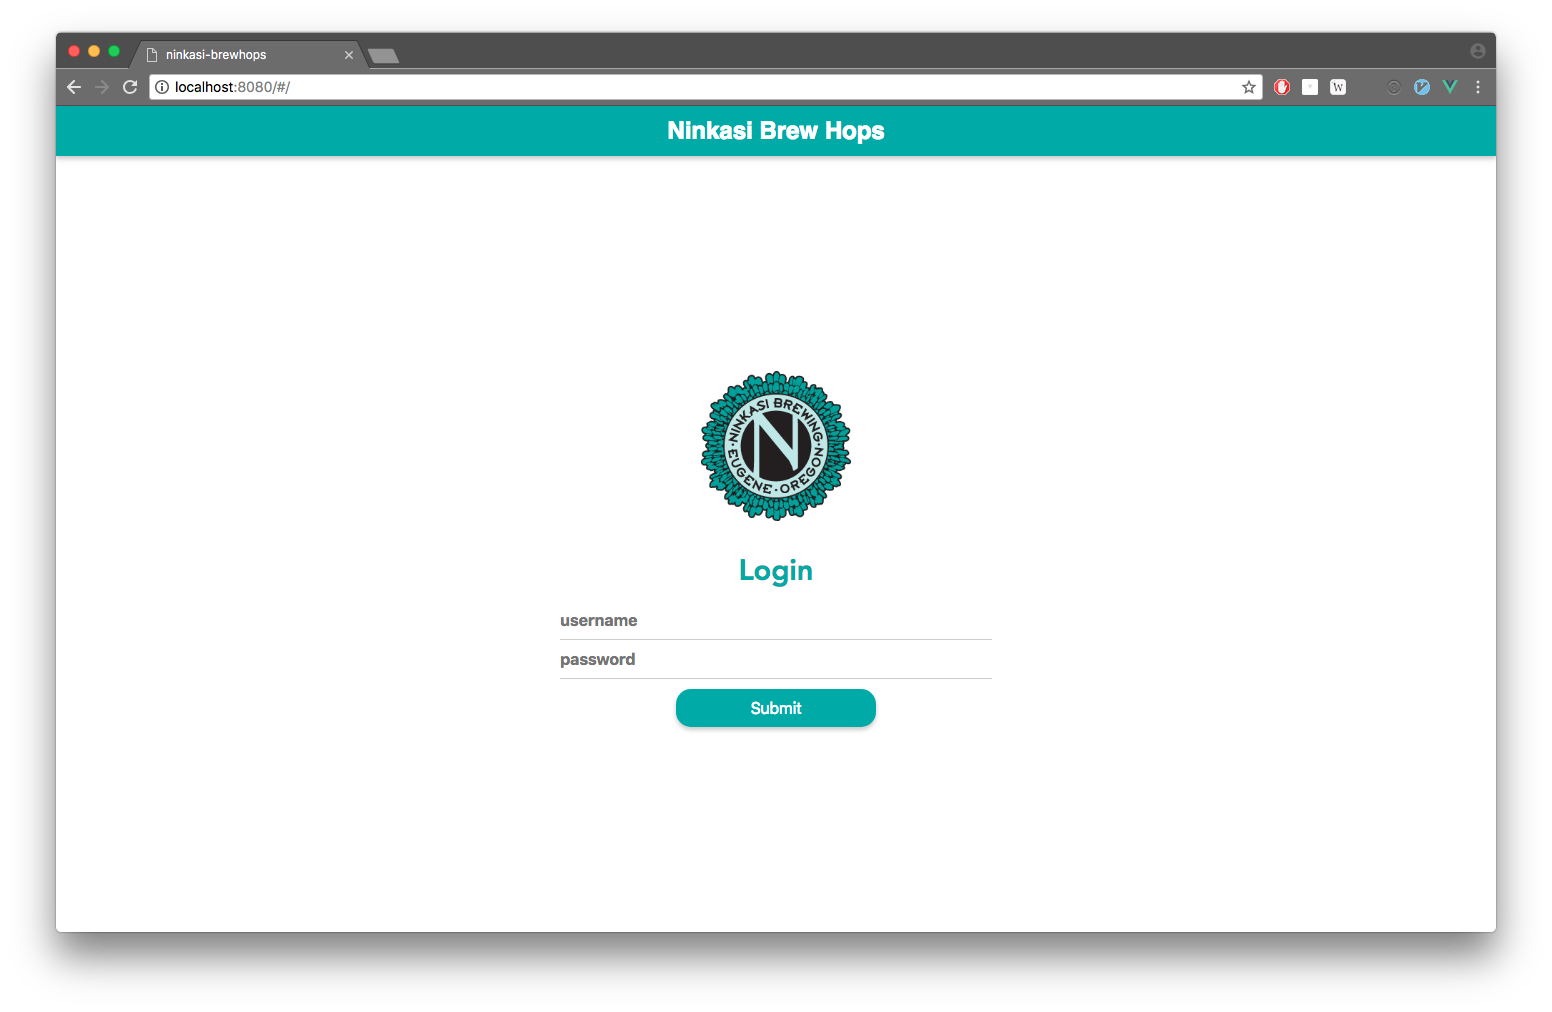
\includegraphics[height=10cm]{screenshots/desktop/login.png}
  \caption{Login page on desktop}
\end{figure}
\begin{figure}
  \centering
  \centerline{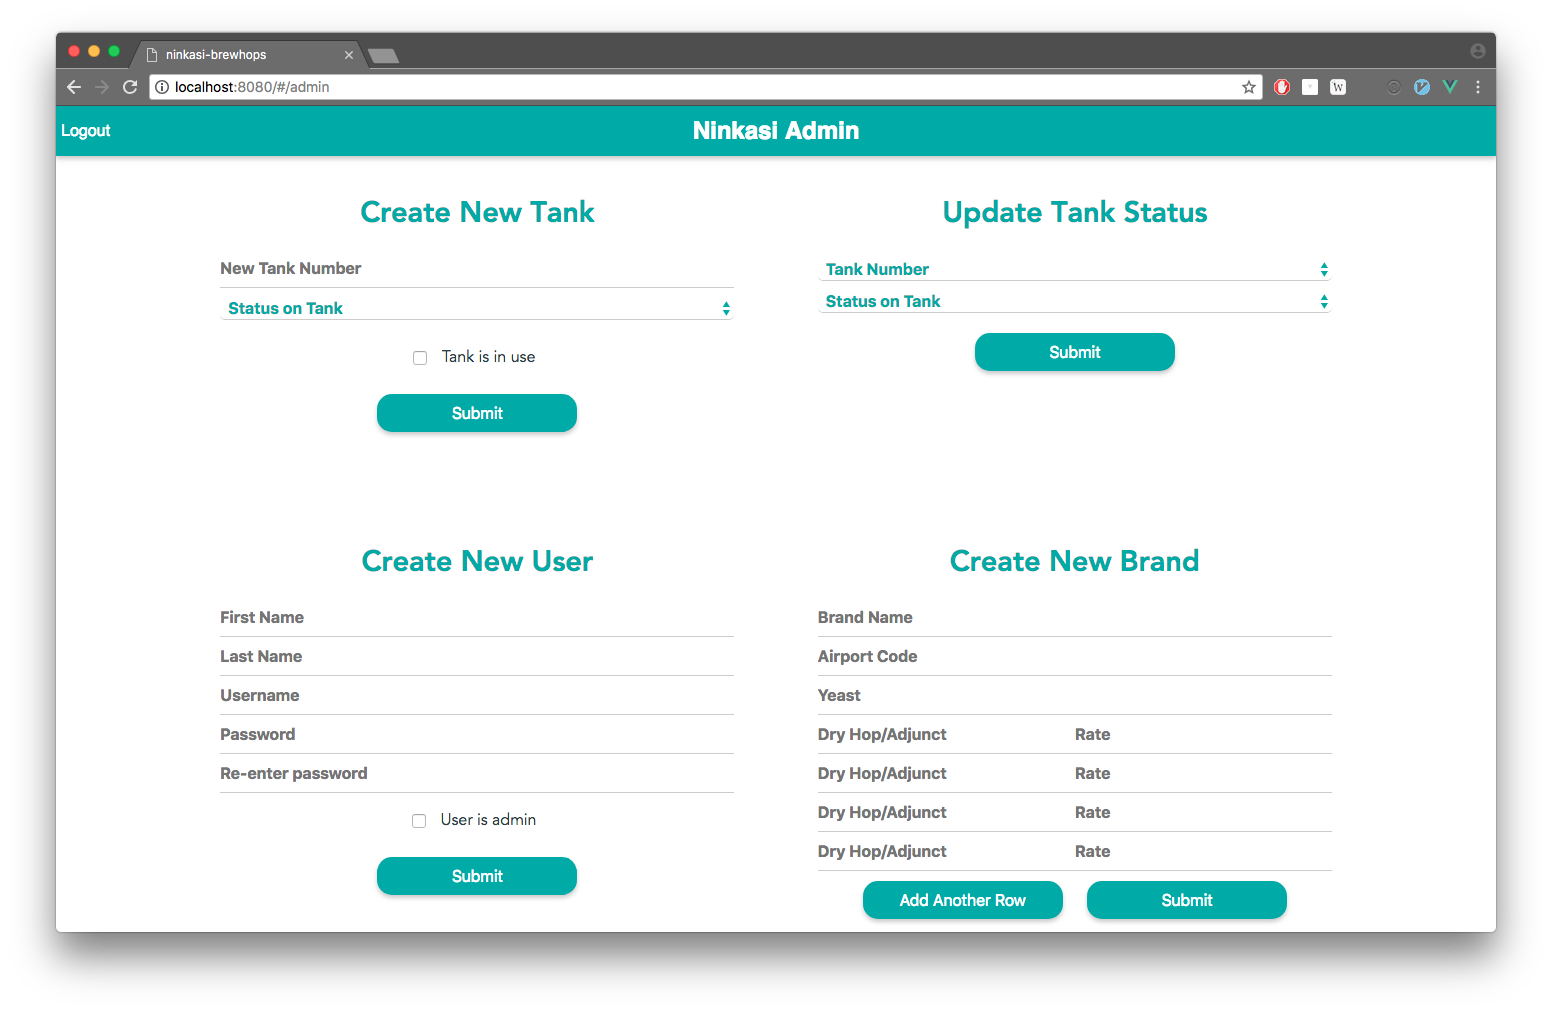
\includegraphics[height=10cm]{screenshots/desktop/admin.png}}
  \caption{Admin page on desktop}
\end{figure}
\begin{figure}
  \centering
  \centerline{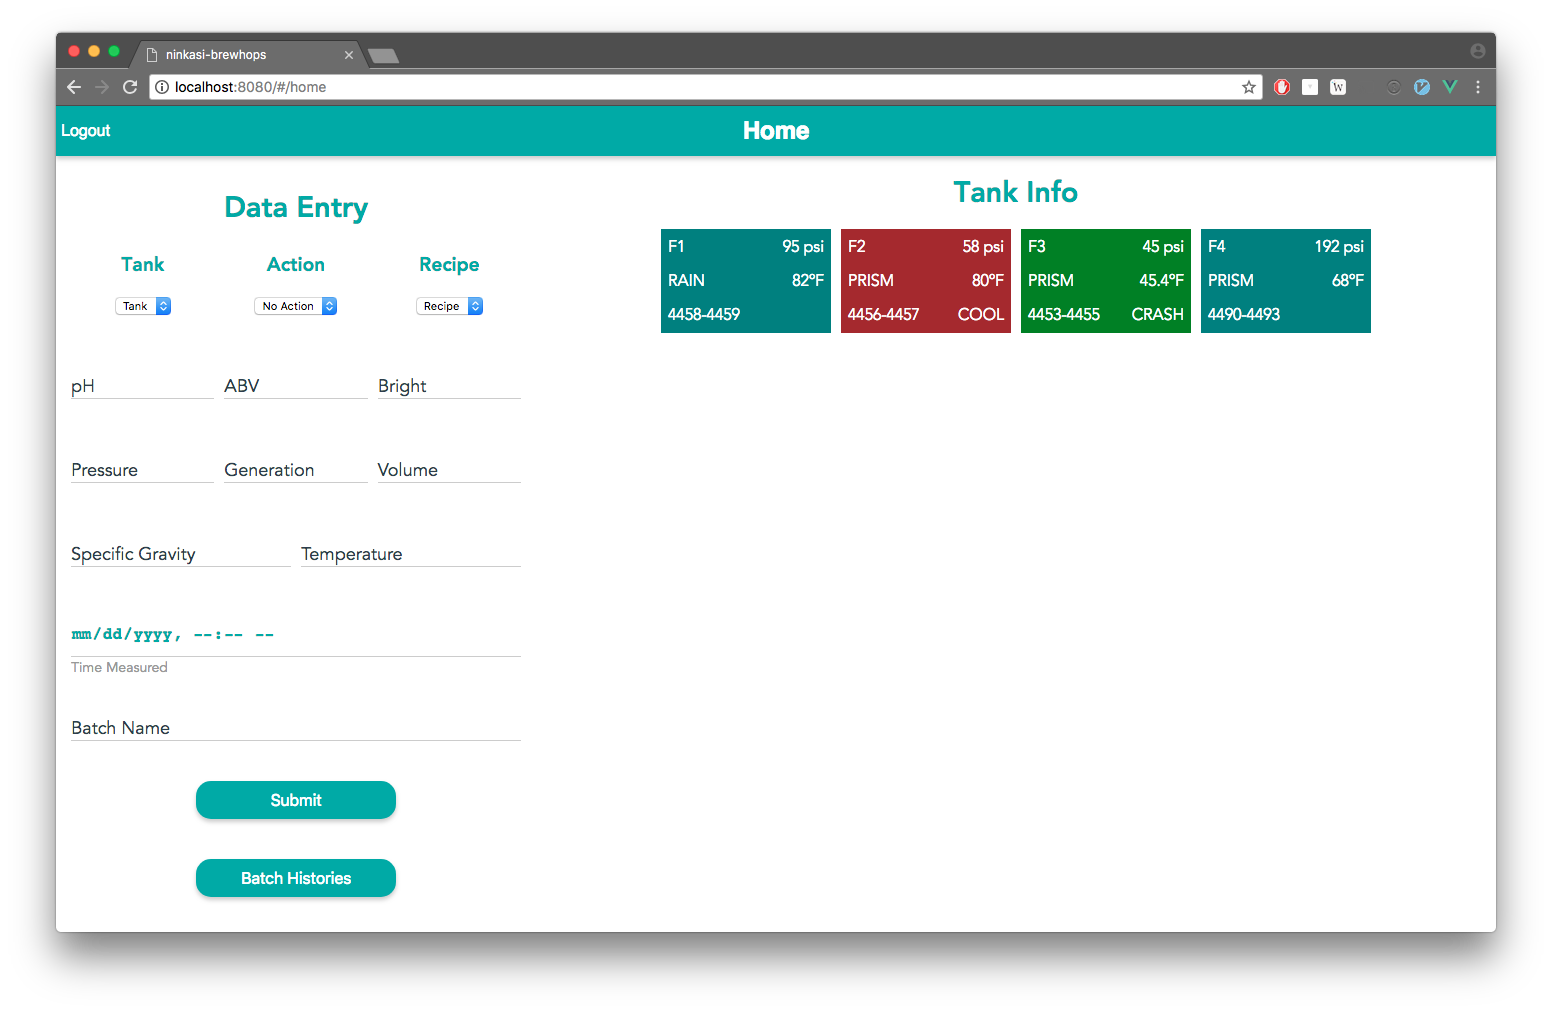
\includegraphics[height=10cm]{screenshots/desktop/home.png}}
  \caption{Home page on desktop}
\end{figure}
\begin{figure}
  \centering
  \centerline{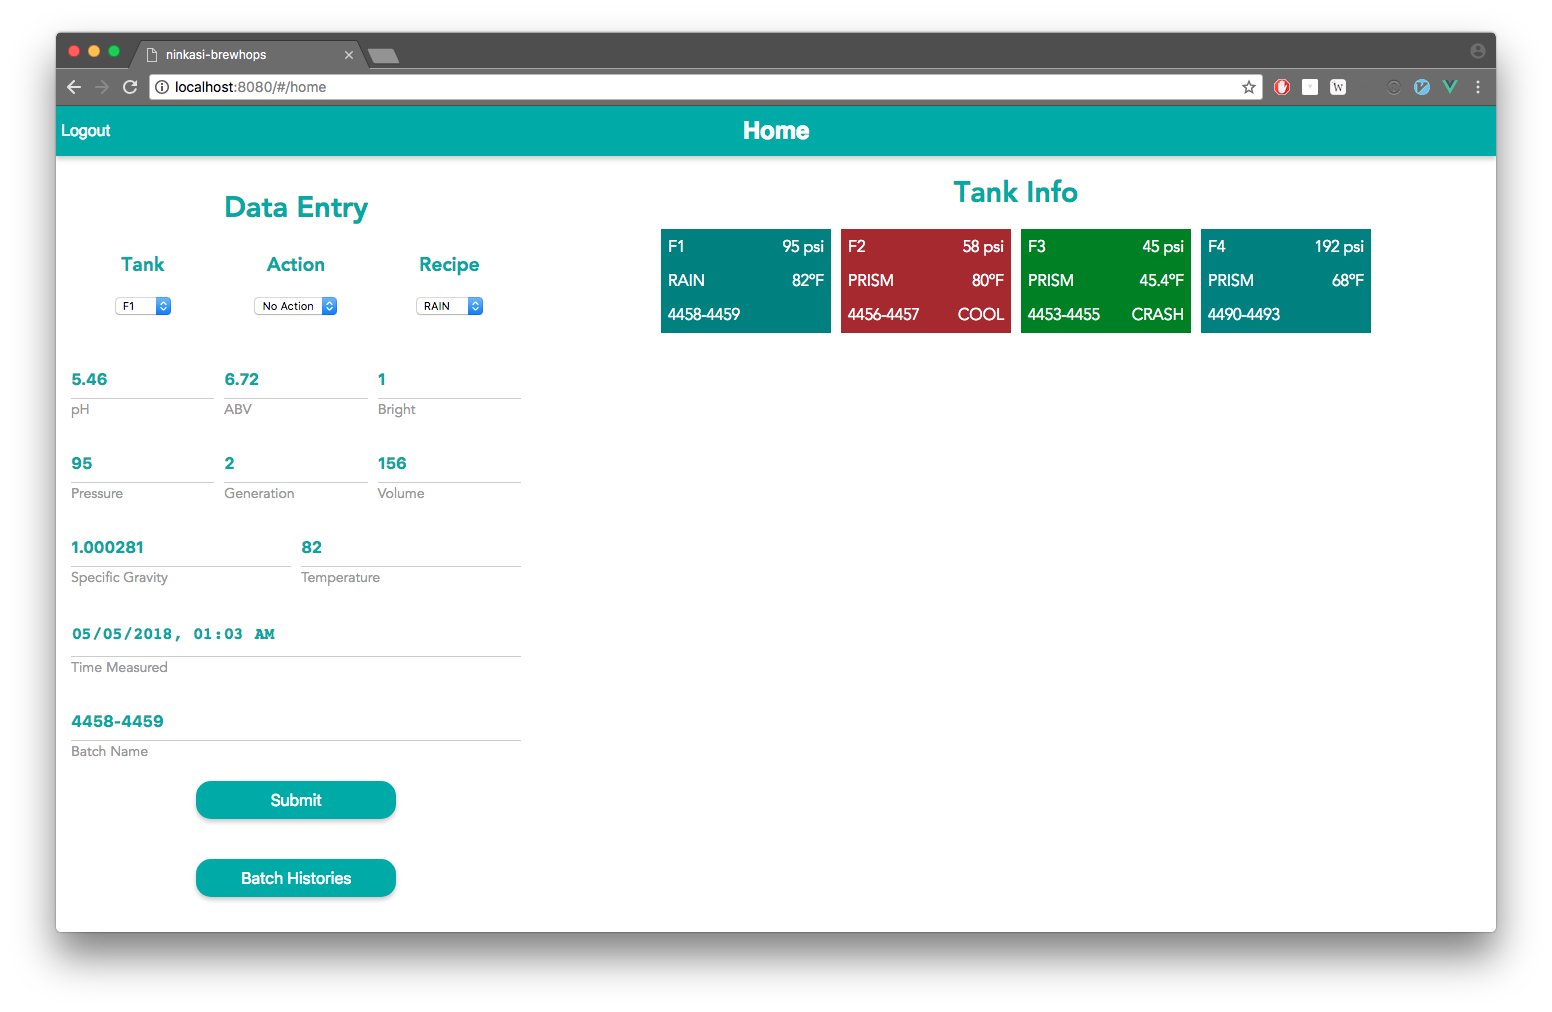
\includegraphics[height=10cm]{screenshots/desktop/home_filled.png}}
  \caption{Home page on desktop with filled content in the data entry component}
\end{figure}
\begin{figure}
  \centering
  \centerline{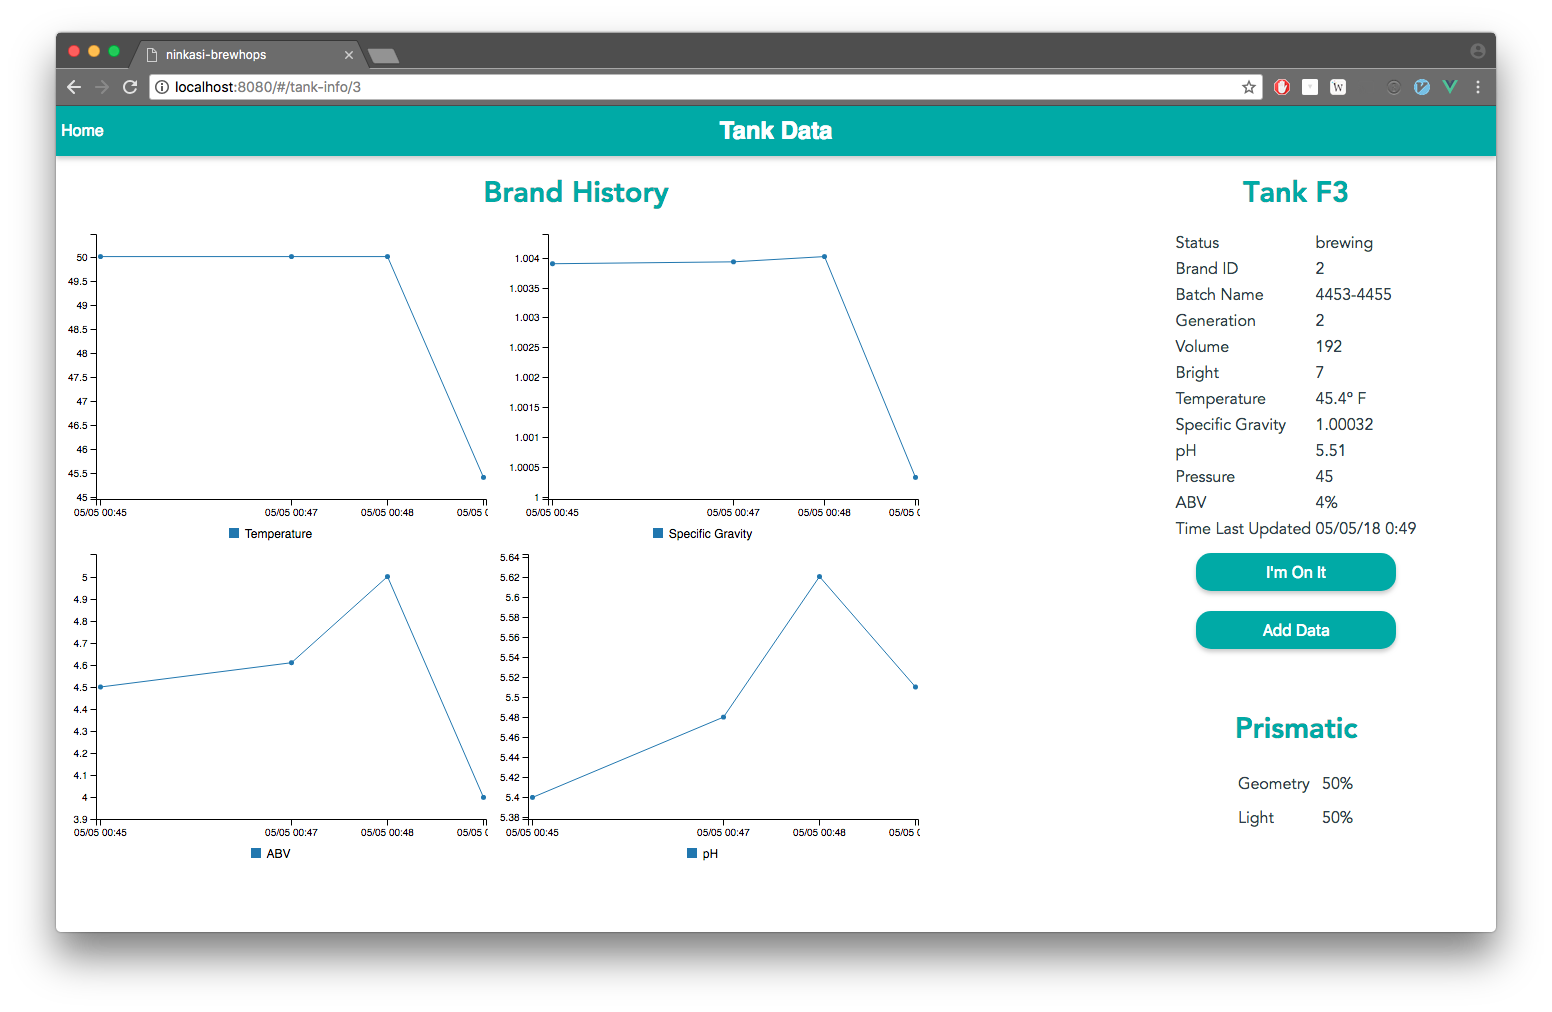
\includegraphics[height=10cm]{screenshots/desktop/tank_info.png}}
  \caption{Tank info page on desktop}
\end{figure}
\begin{figure}
  \centering
  \centerline{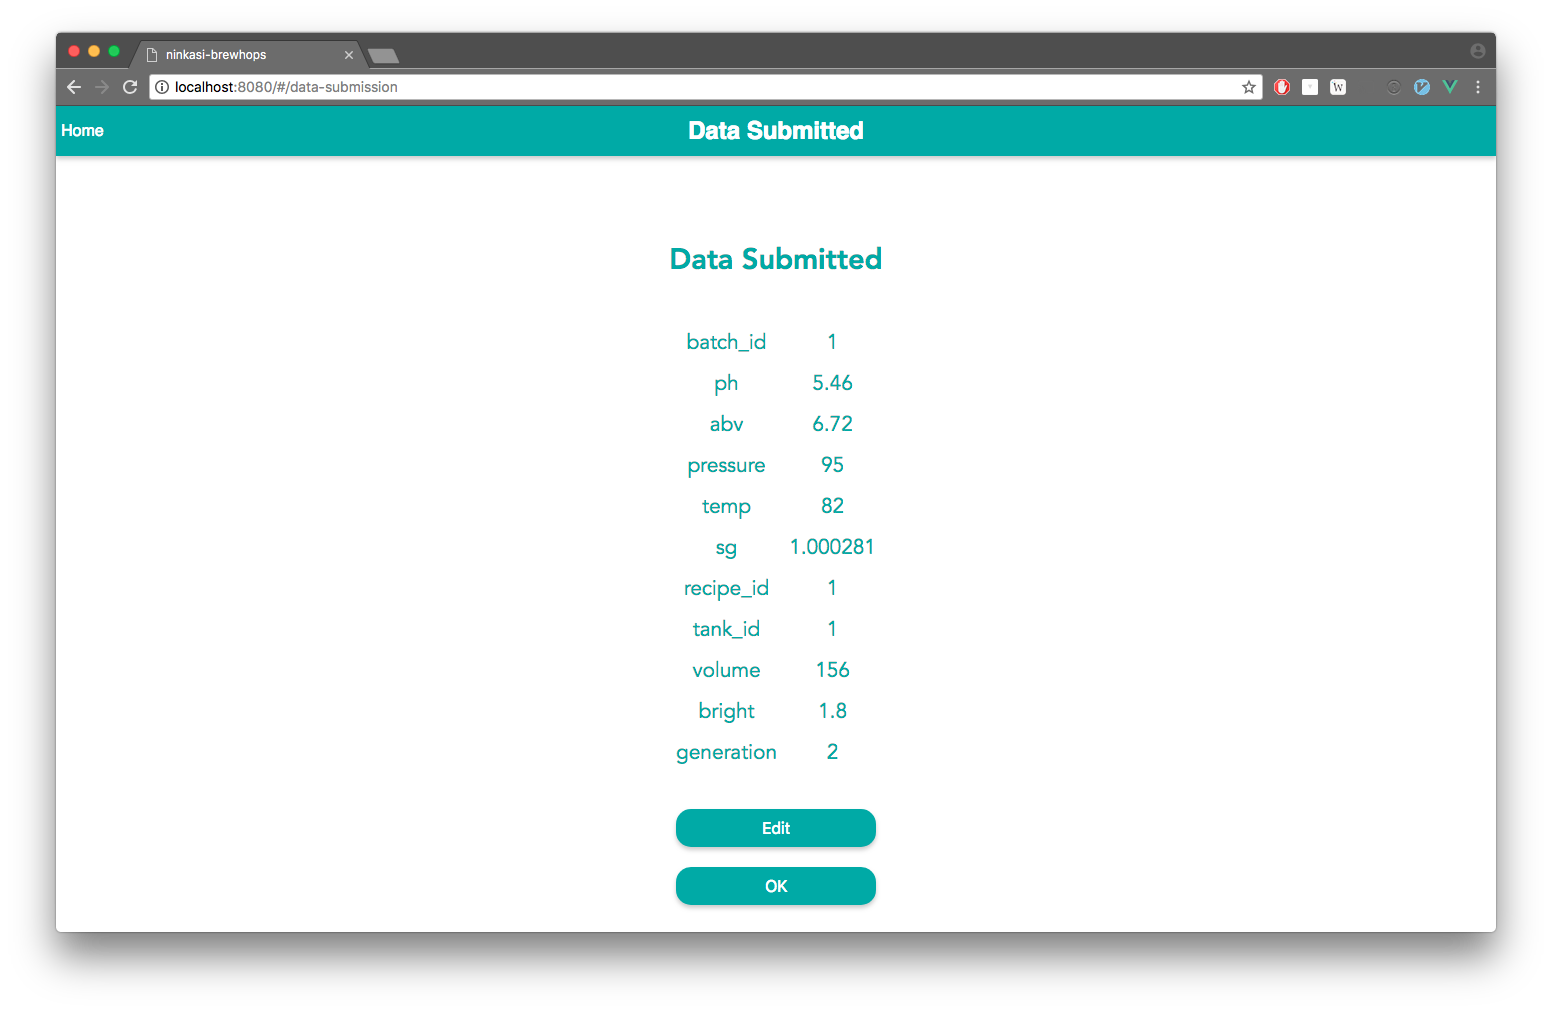
\includegraphics[height=10cm]{screenshots/desktop/data_submission.png}}
  \caption{Data submission page on desktop}
\end{figure}

\begin{figure}
  \centering
  \centerline{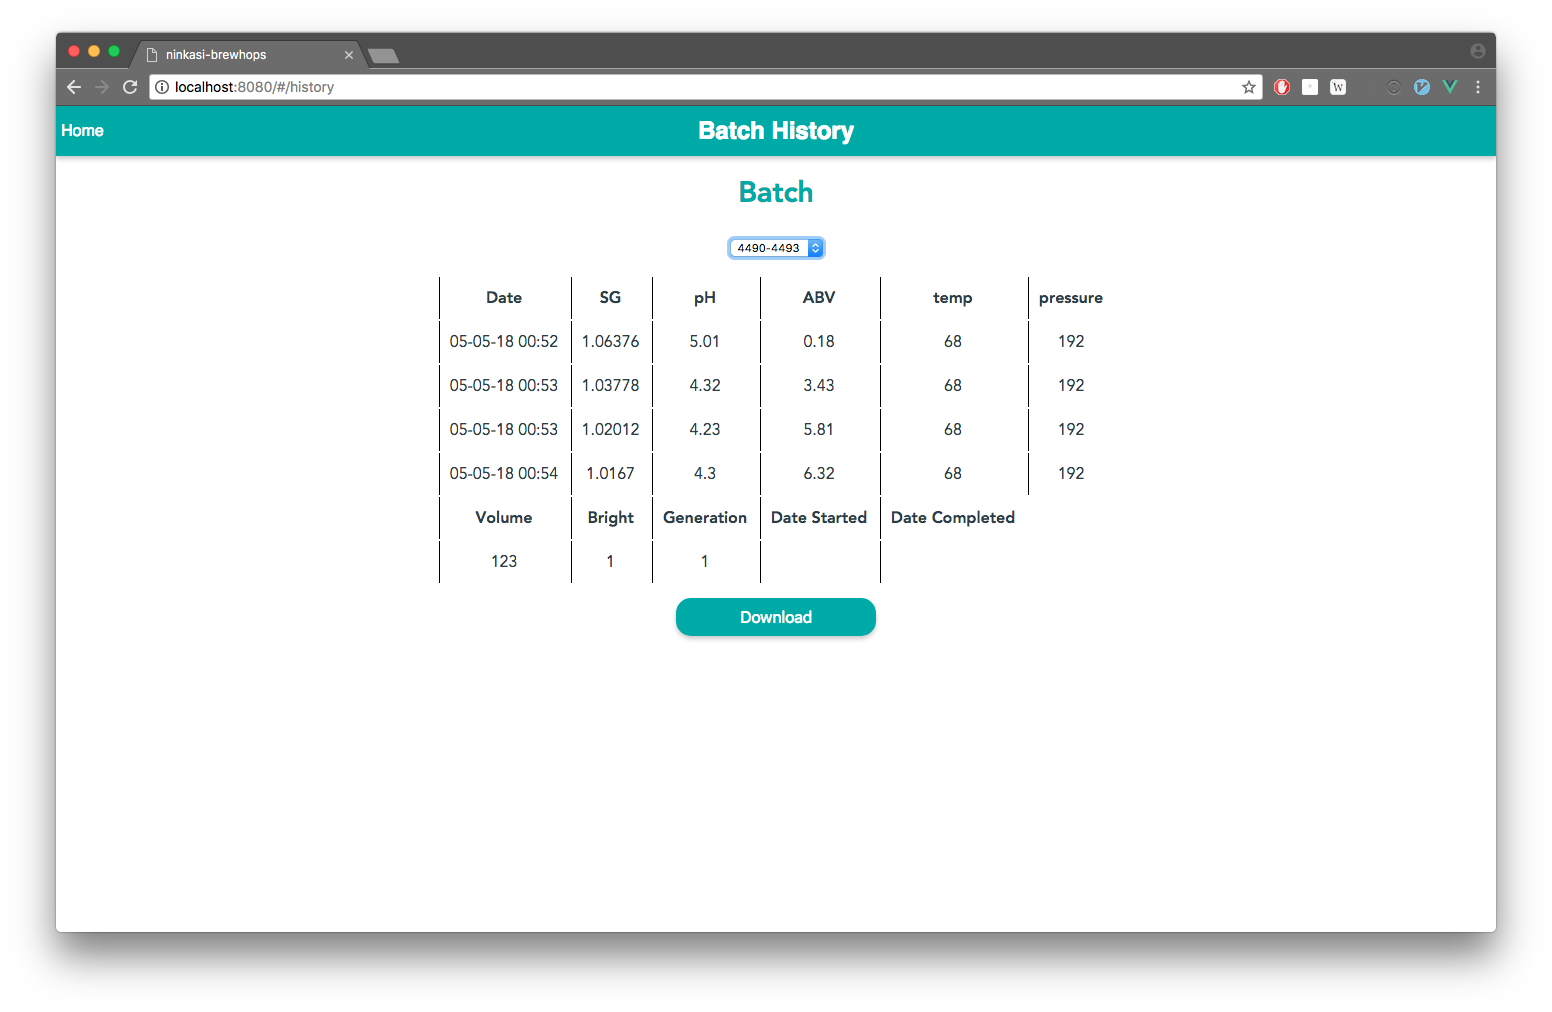
\includegraphics[height=10cm]{screenshots/desktop/batch_history.png}}
  \caption{Batch history page on desktop}
\end{figure}
\begin{figure}
  \centering
  \centerline{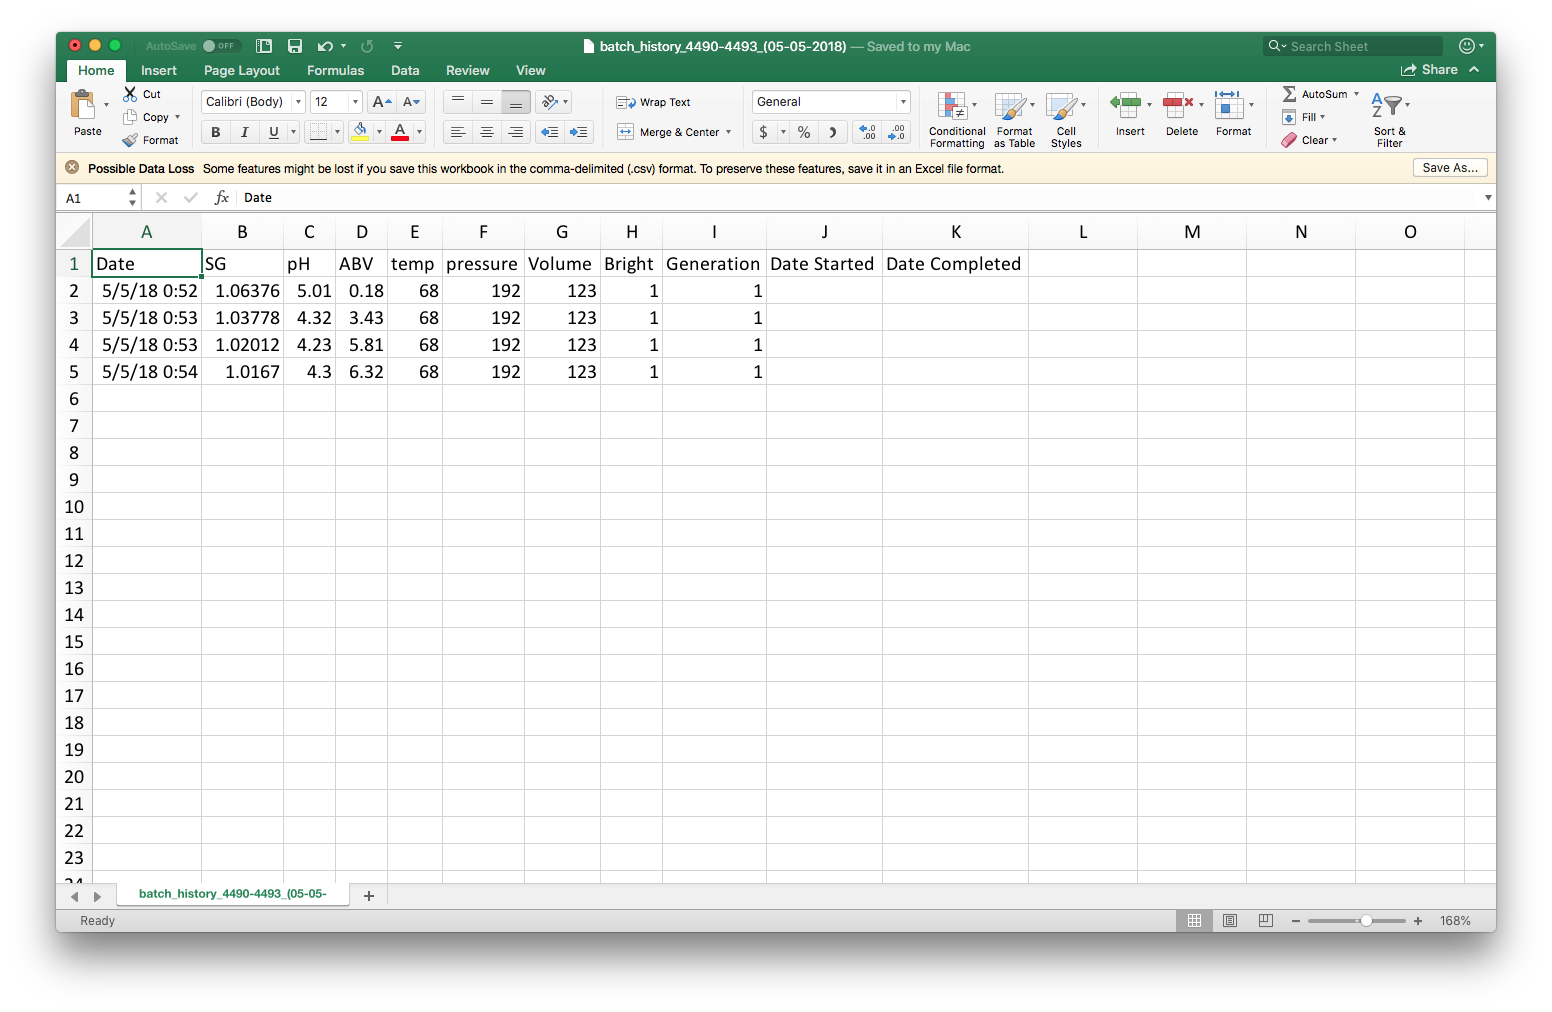
\includegraphics[height=10cm]{screenshots/desktop/csv.png}}
  \caption{The downloaded information from the batch history page in a csv}
\end{figure}


\begin{figure}%
    \centering
    \subfloat[Login]{{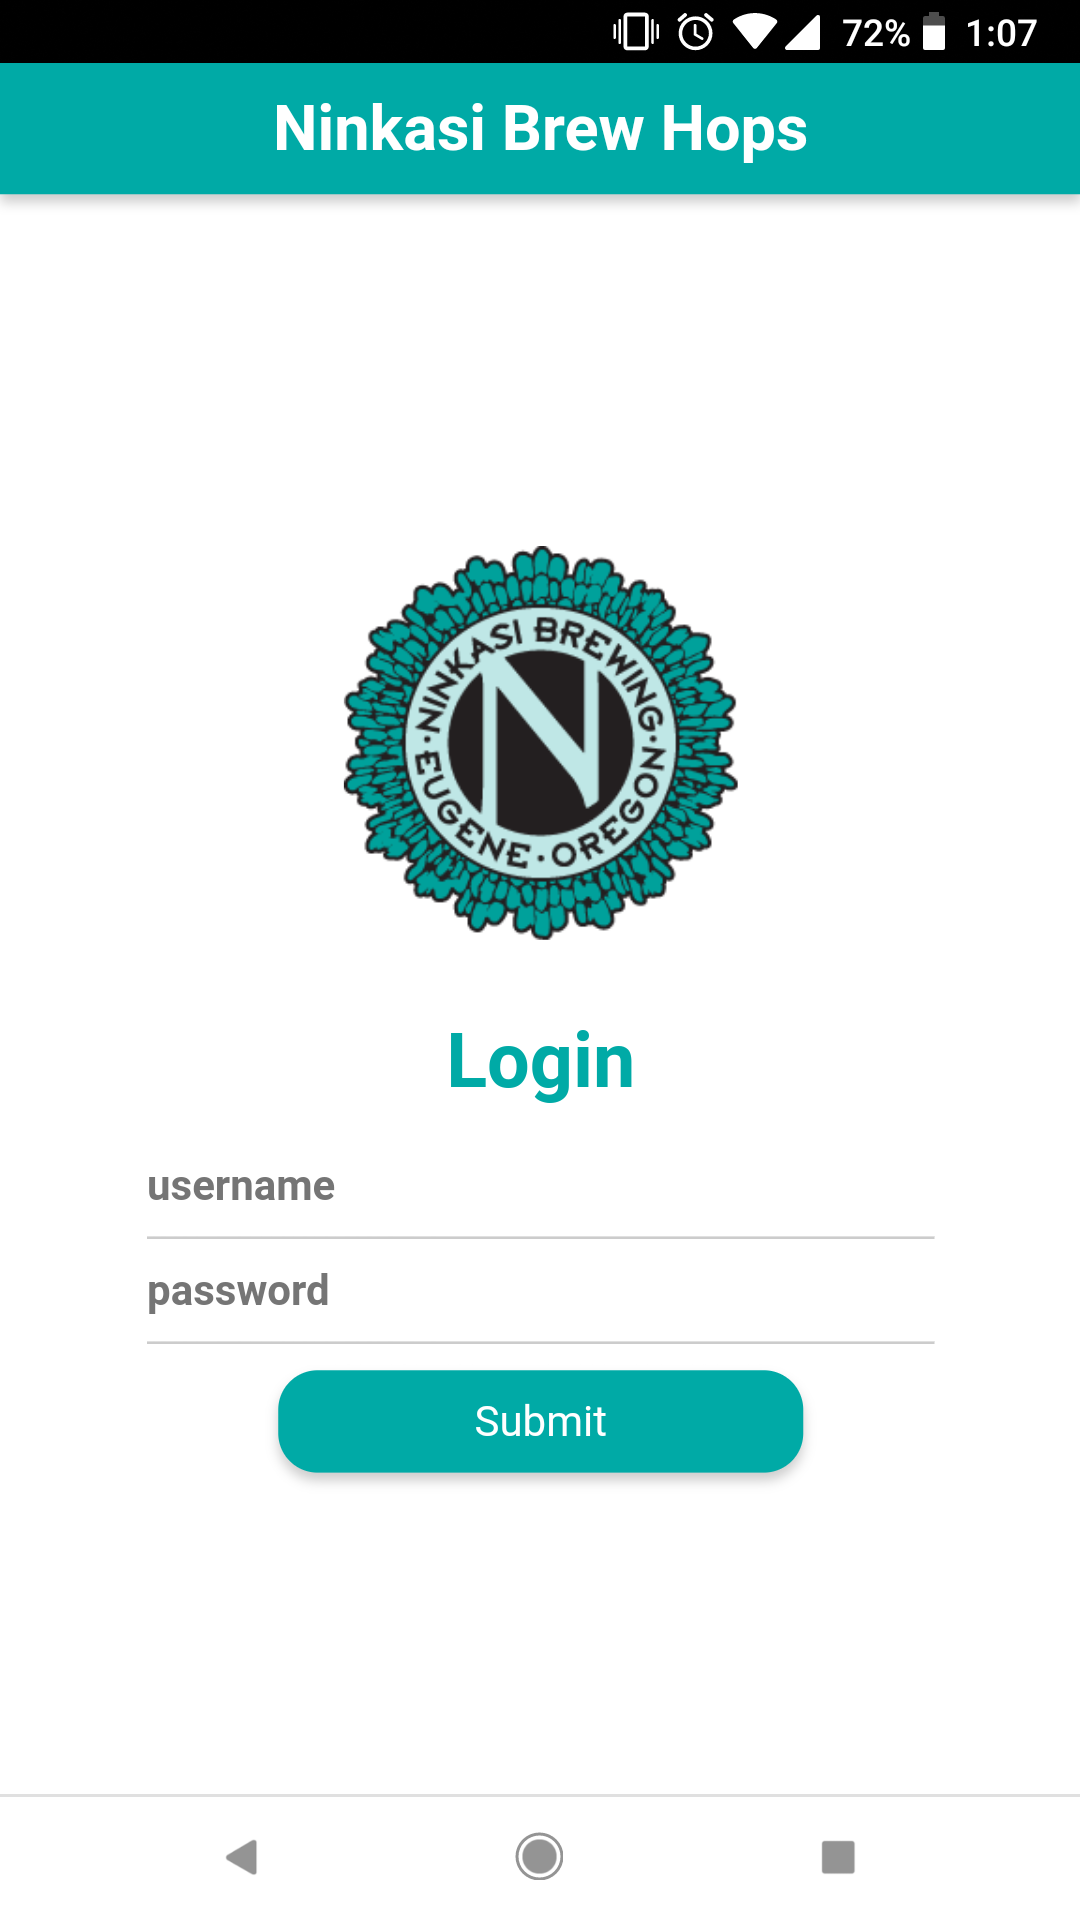
\includegraphics[height=13cm]{screenshots/mobile/login.png}}}%
    \qquad
    \subfloat[Home]{{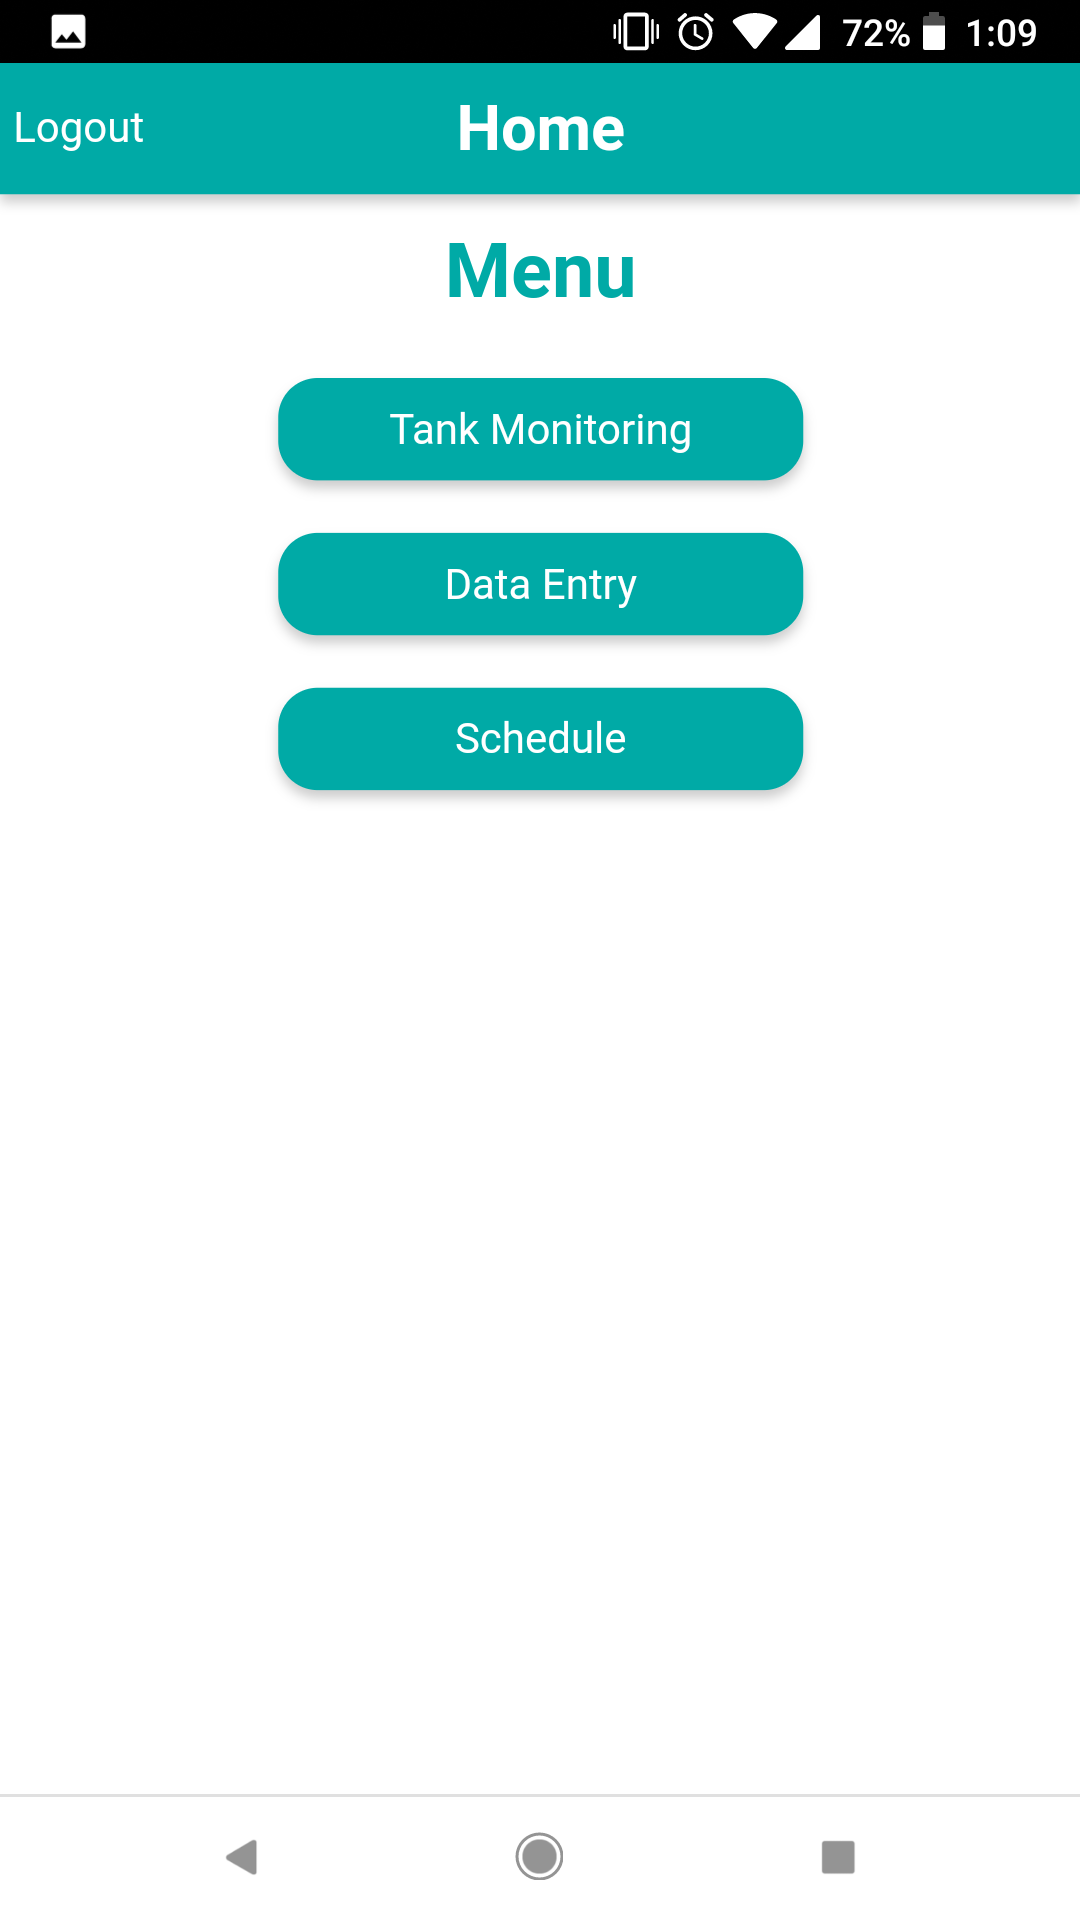
\includegraphics[height=13cm]{screenshots/mobile/home.png}}}%
    \caption{Mobile - Login and Home page}%
\end{figure}

\begin{figure}%
    \centering
    \subfloat[Tank Monitoring]{{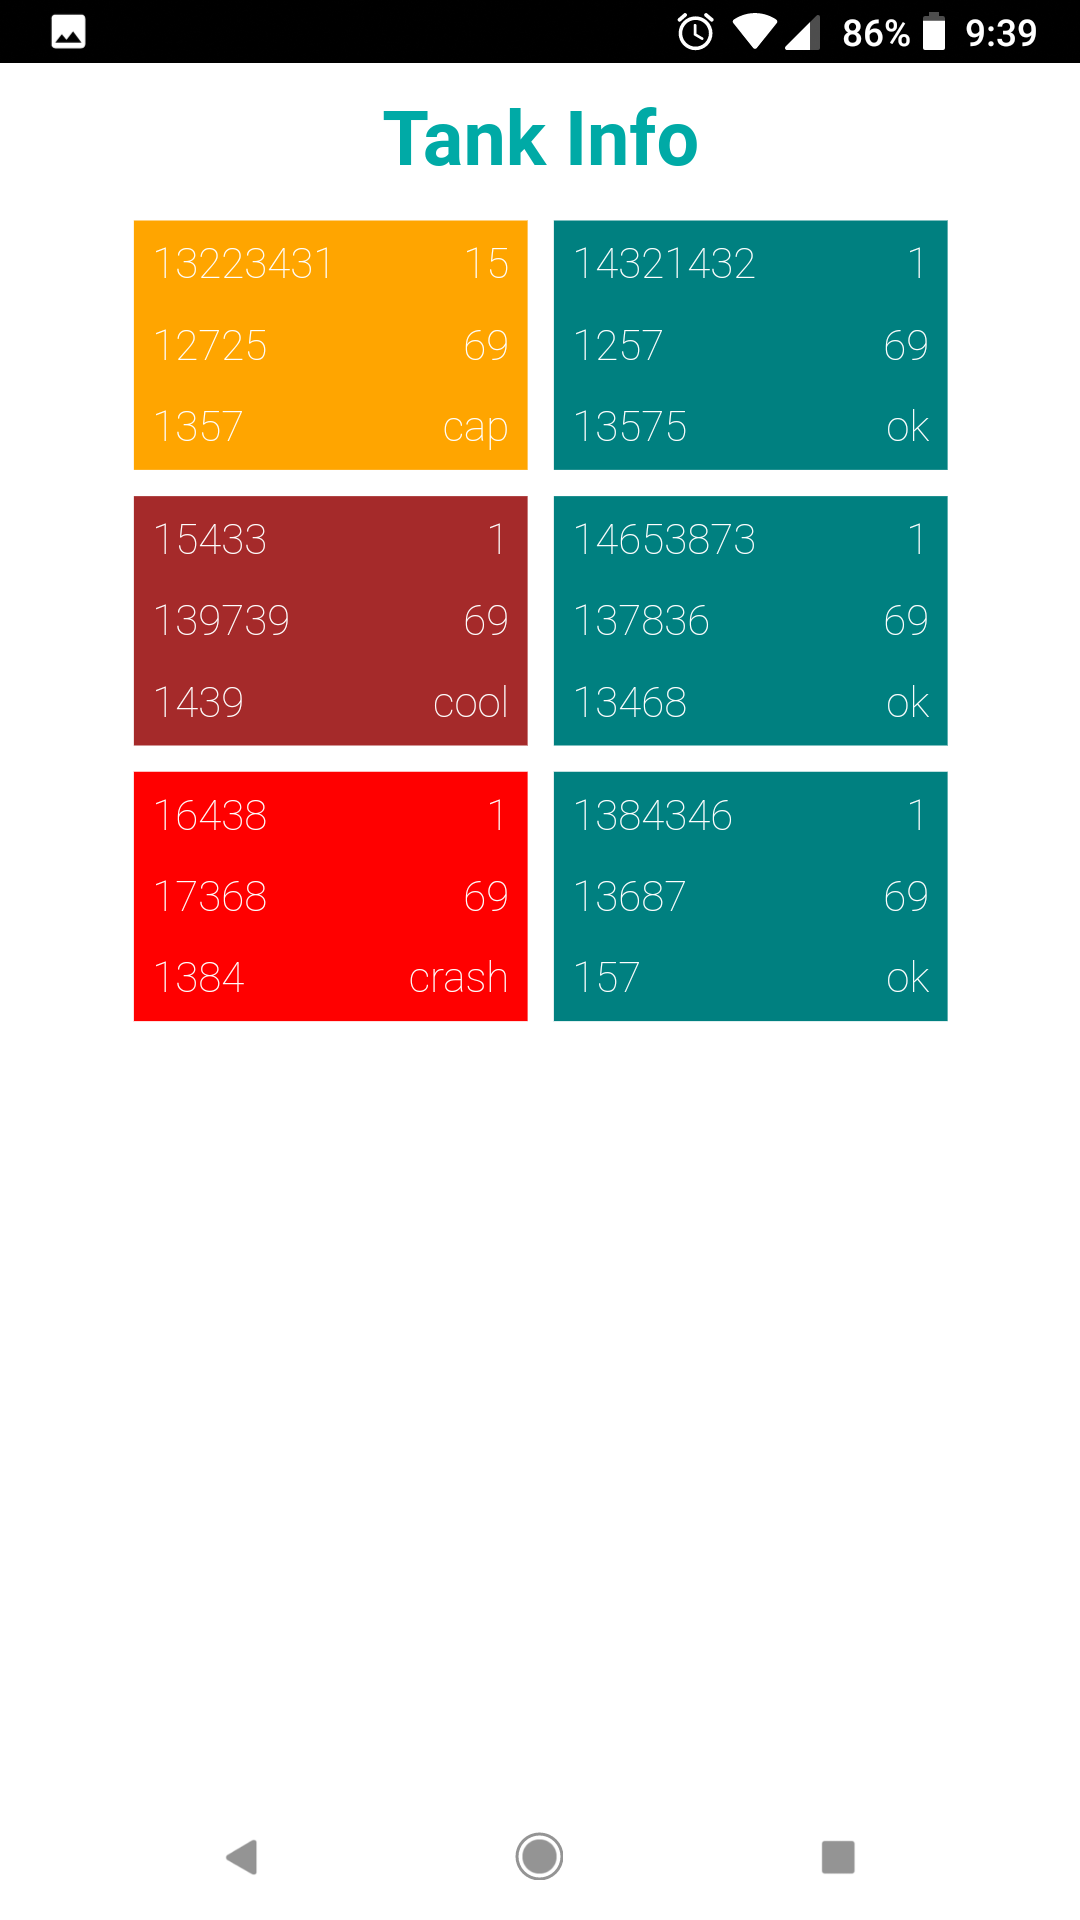
\includegraphics[height=13cm]{screenshots/mobile/tank_monitoring.png}}}%
    \qquad
    \subfloat[Tank Info]{{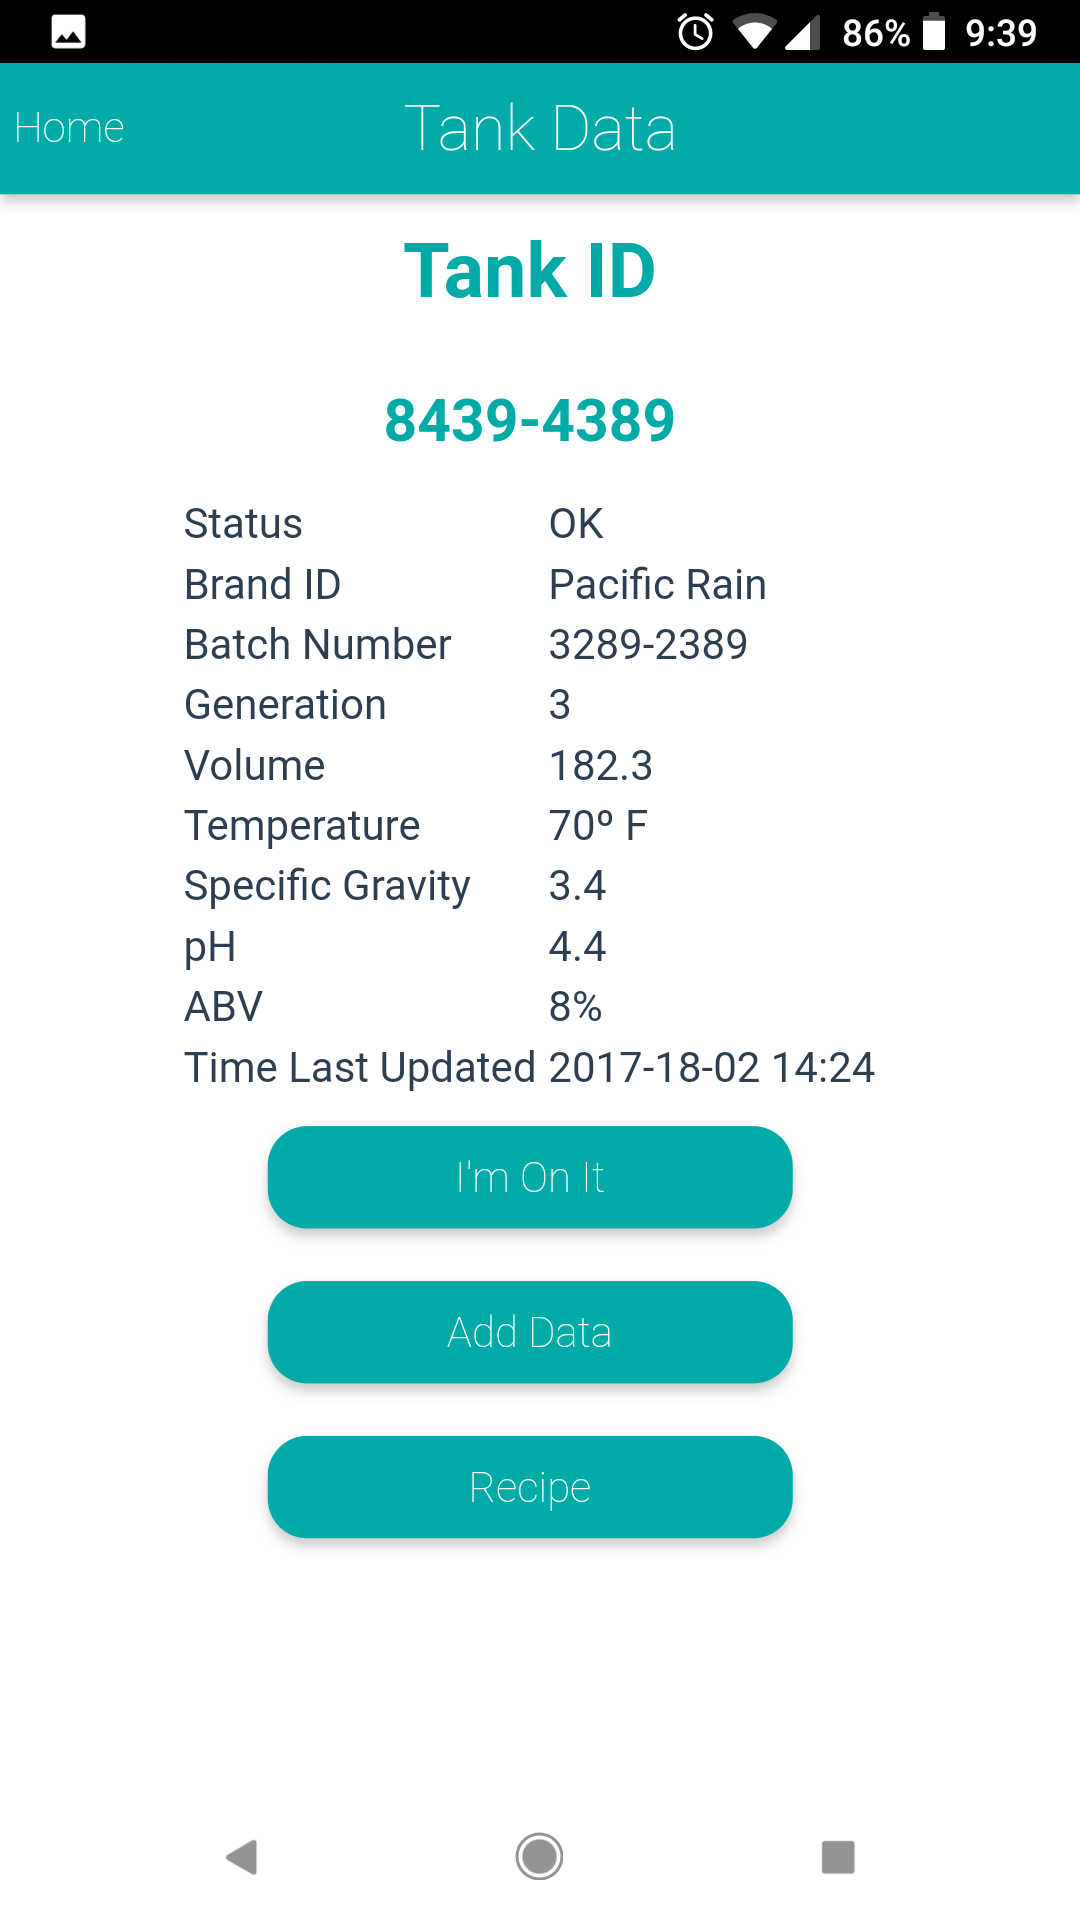
\includegraphics[height=13cm]{screenshots/mobile/tank_info.png}}}%
    \caption{Mobile - Tank monitoring and more info page}%
\end{figure}

\begin{figure}
	\centering
	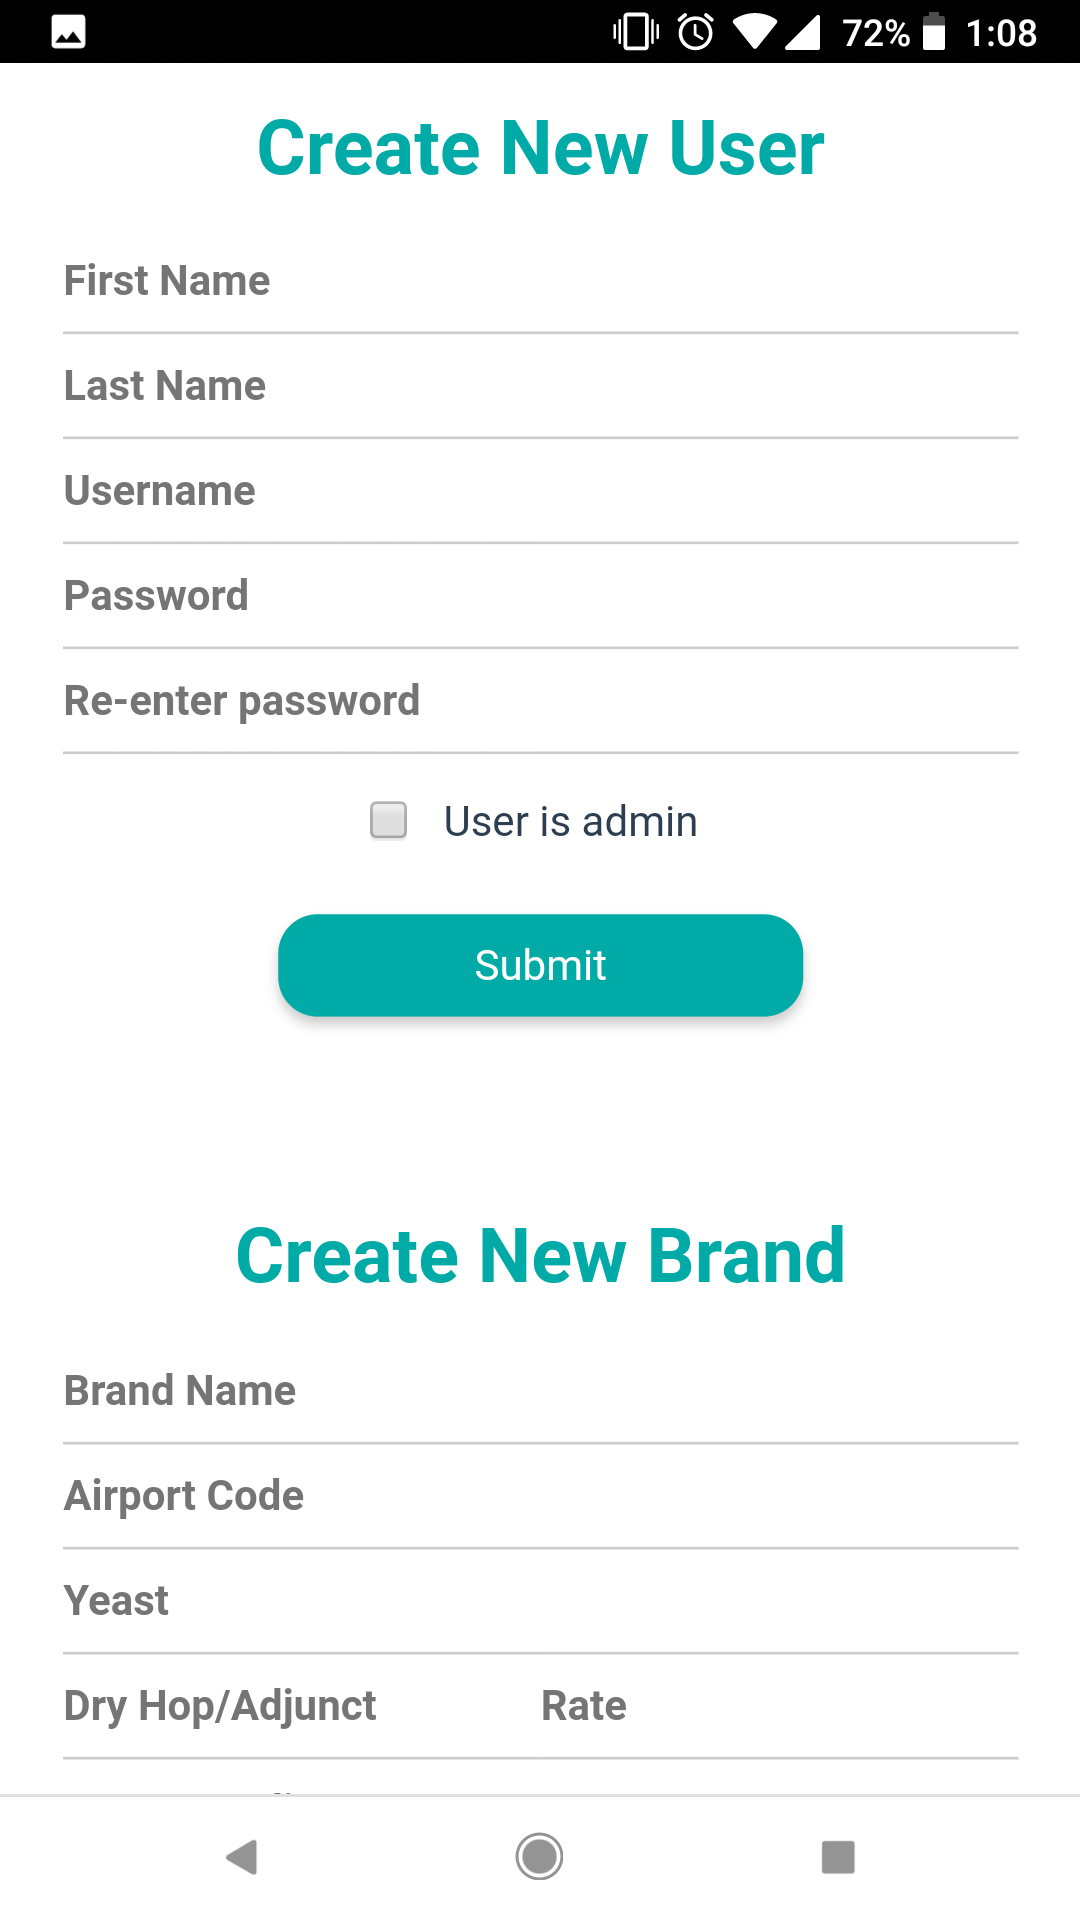
\includegraphics[height=13cm]{screenshots/mobile/admin.png}
  \caption{Admin page on mobile}
\end{figure}

\begin{figure}%
    \centering
    \subfloat[Data Entry]{{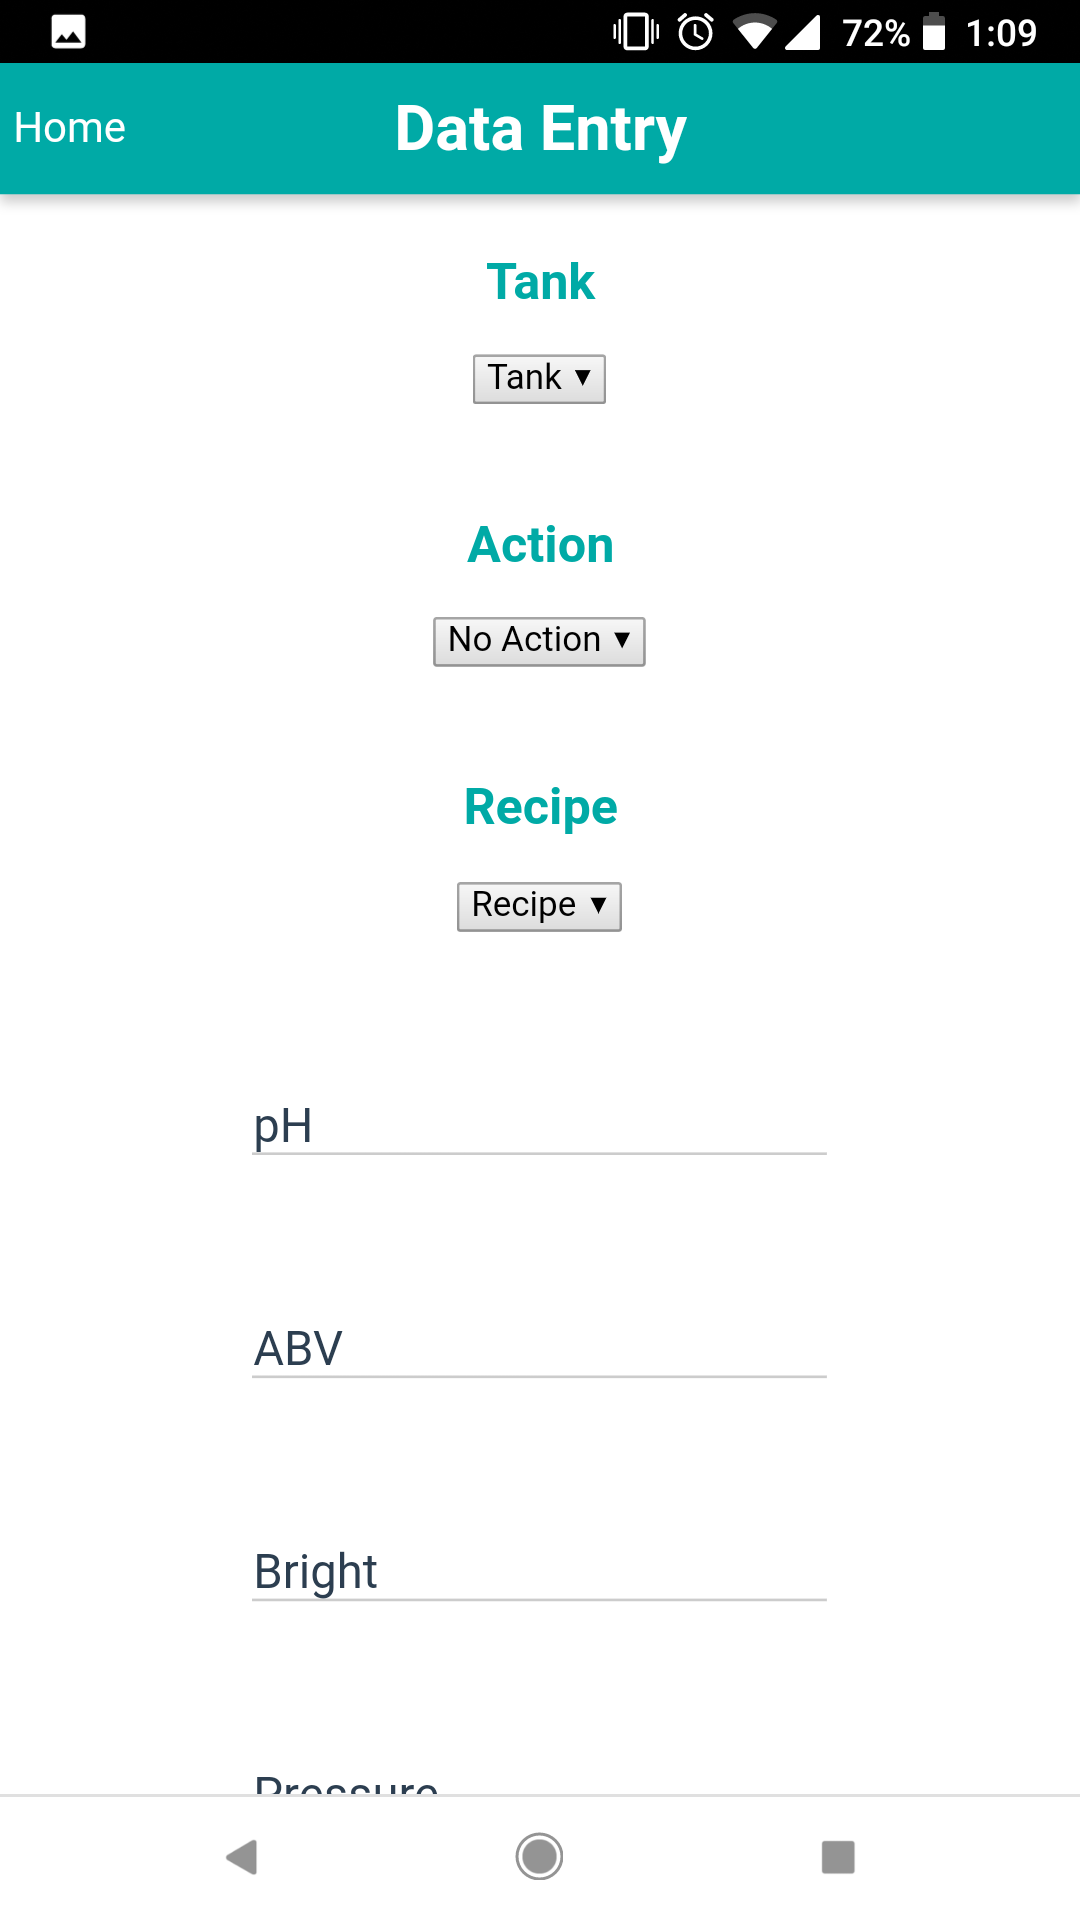
\includegraphics[height=13cm]{screenshots/mobile/data_entry.png}}}%
    \qquad
    \subfloat[Submission]{{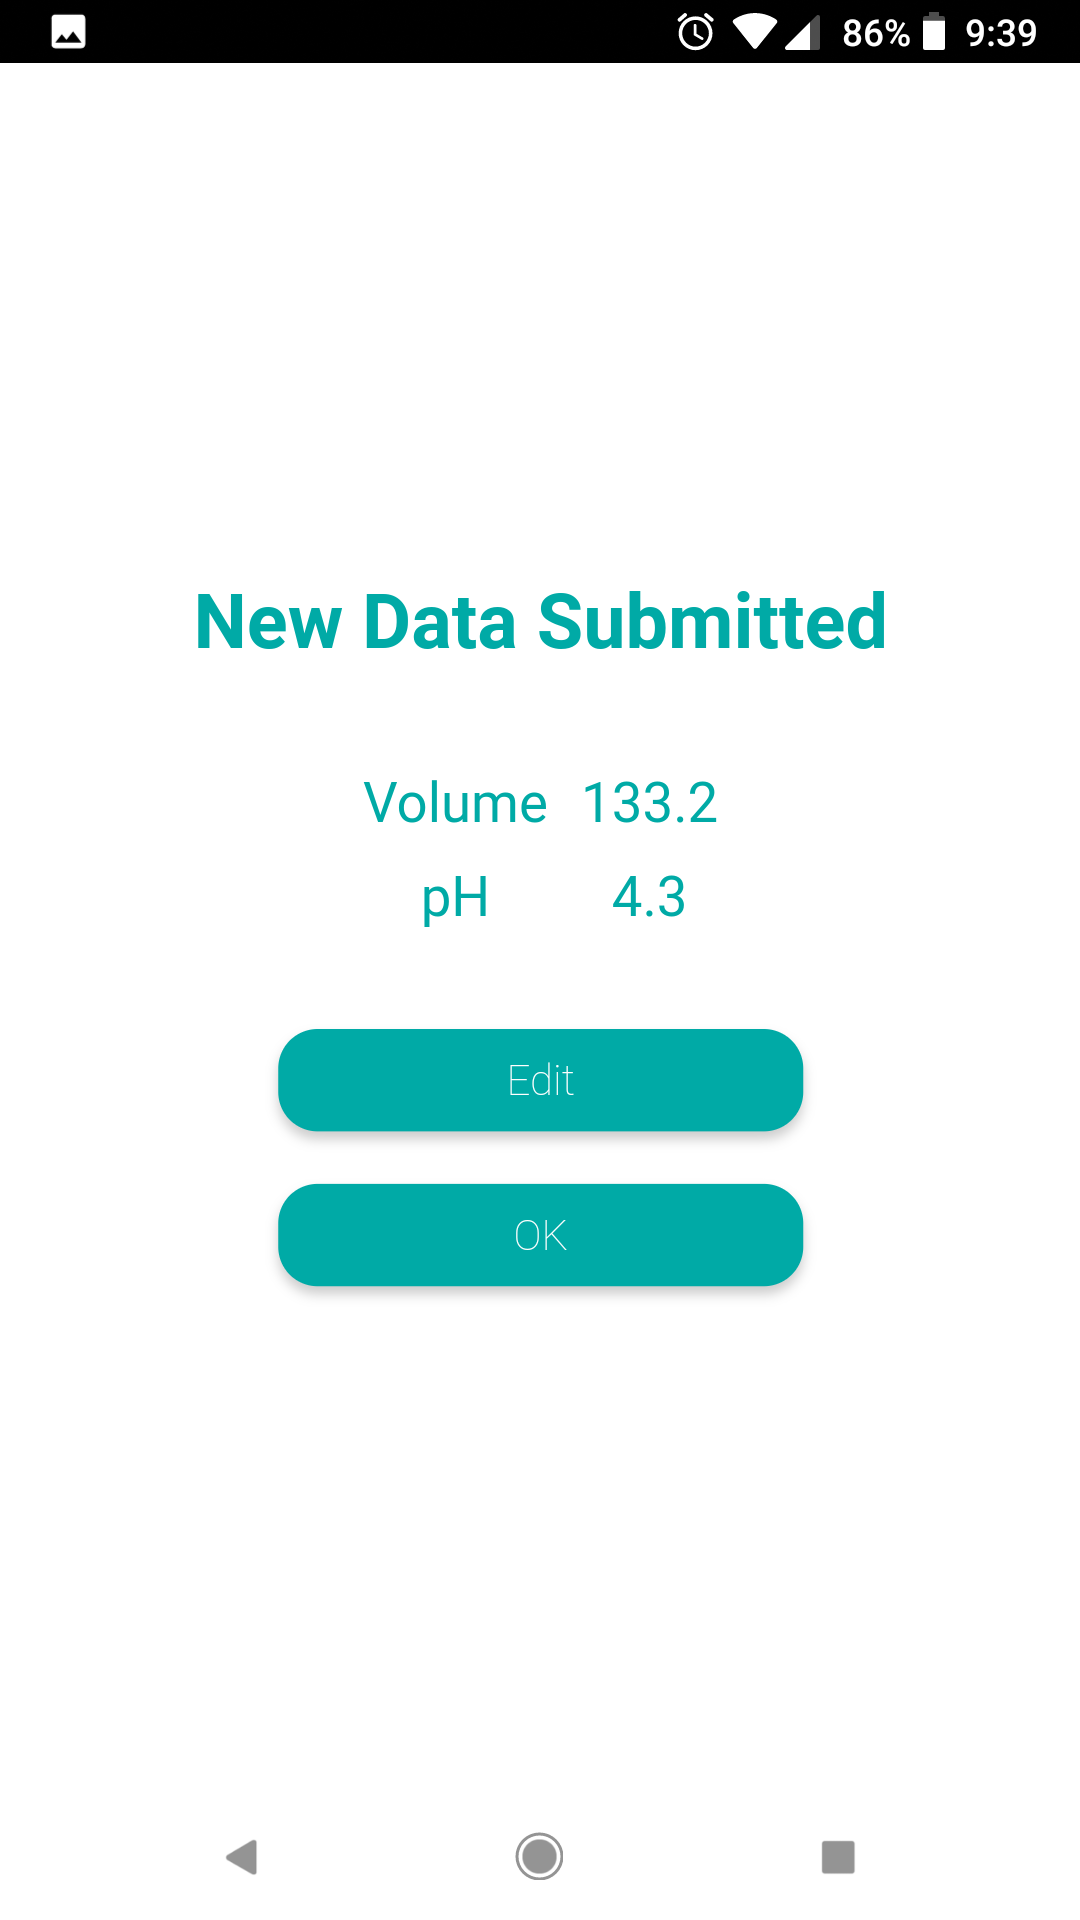
\includegraphics[height=13cm]{screenshots/mobile/submission.png}}}
    \caption{Mobile - Data entry and submission pages}%
\end{figure}

\end{document}
